
\chapter{Risultati}
Per poter definire l'efficenza e l'effettiva scabilità del sistema creato 
è stato necessario metterlo alla prova. 
A questo fine, vengono eseguiti dei test che comportano un elevato carico di richieste,
per misurare le prestazioni in momenti di grande utilizzo e
verificare che sia così garantita la qualità del servizio anche sotto stress.\\
\\
Nell'ottica di ottenere dei risultati che descrivano fedelmente 
il comportamento dell'applicazione,
sono state selezionate alcune funzionalità,
in base sia alla loro centralità nel comportamento del sistema,
che alla loro complessità di coordinamento dei componenti dell'applicazione.
quali\\

come
\section{L'impostazione dei test}

\section{Velocità in lettura}
perchè è stata scelta
cosa comporta la funzione(come funziona sotto)
come faccio questo test
grafici
interpretazione dei risultati
\section{Velocità in creazione}
\section{Velocità degli aggiornamenti}
\section{Garanzia della propagazione delle informazioni}
\section{Velocità di upload delle immagini}


\section{Velocità in lettura}

\begin{figure}[htbp]
    \begin{center}
        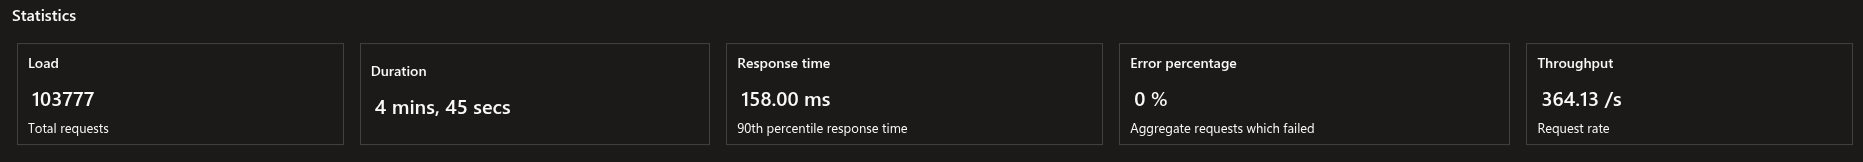
\includegraphics[width=\textwidth]{TestLettura1.png}
        \caption{158 ms su una media di 364 richieste al secondo}
    \end{center}
\end{figure}

\begin{figure}[htbp]
    \begin{center}
        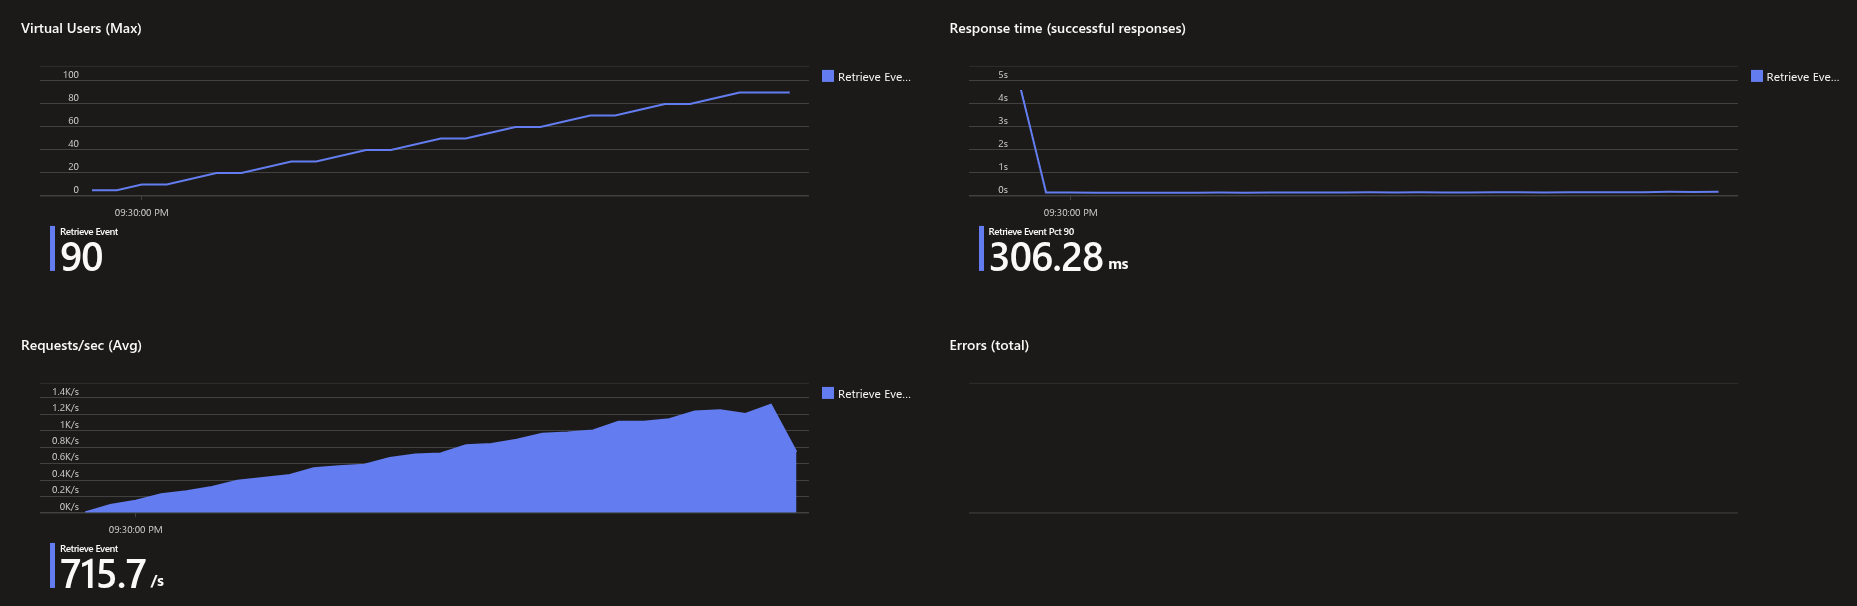
\includegraphics[width=\textwidth]{TestLettura2.png}
        \caption{il tempo di risposta non varia in base al numero di richieste}
    \end{center}
\end{figure}

\begin{figure}[htbp]
    \begin{center}
        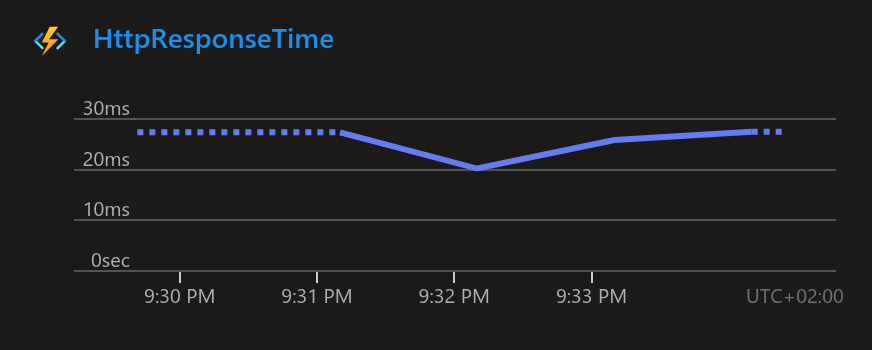
\includegraphics[width=\textwidth]{TestLettura3.png}
        \caption{Dettaglio della velocità senza tempo di trasmissione}
    \end{center}
\end{figure}
\clearpage
\section{Caricamento di immagini concorrenti}

\begin{figure}[htbp]
    \begin{center}
        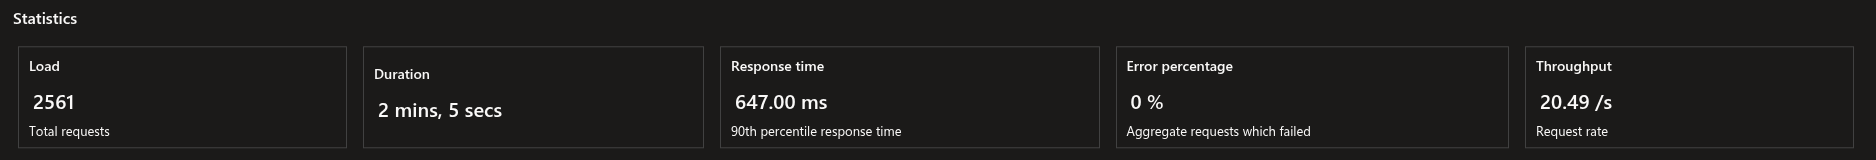
\includegraphics[width=\textwidth]{UploadImages1.png}
        \caption{2 MB di immagini in 600 ms 20 volte al secondo}  
    \end{center}
\end{figure}

\begin{figure}[htbp]
    \begin{center}
        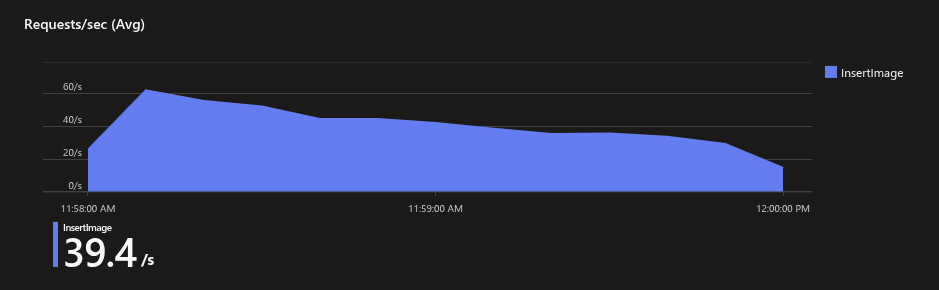
\includegraphics[width=\textwidth]{UploadImages3.png}
        \caption{Andamento delle richieste}  
    \end{center}
\end{figure}

\begin{figure}[htbp]
    \begin{center}
        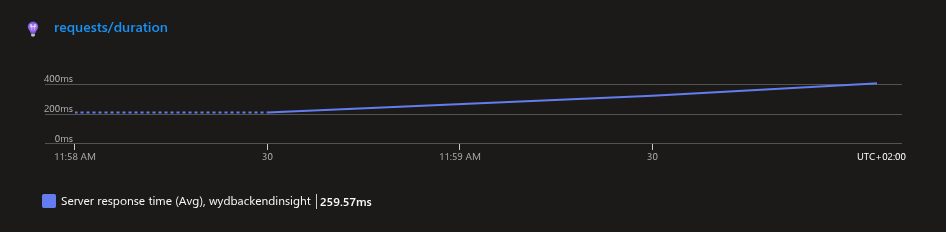
\includegraphics[width=\textwidth]{UploadImages2.png}
        \caption{Dettaglio della velocità richiesta dal server}
    \end{center}
\end{figure}


\clearpage
\chapter*{Conclusione}
\addcontentsline{toc}{chapter}{Conclusione}

\begin{figure}[htbp]
    \begin{center}
        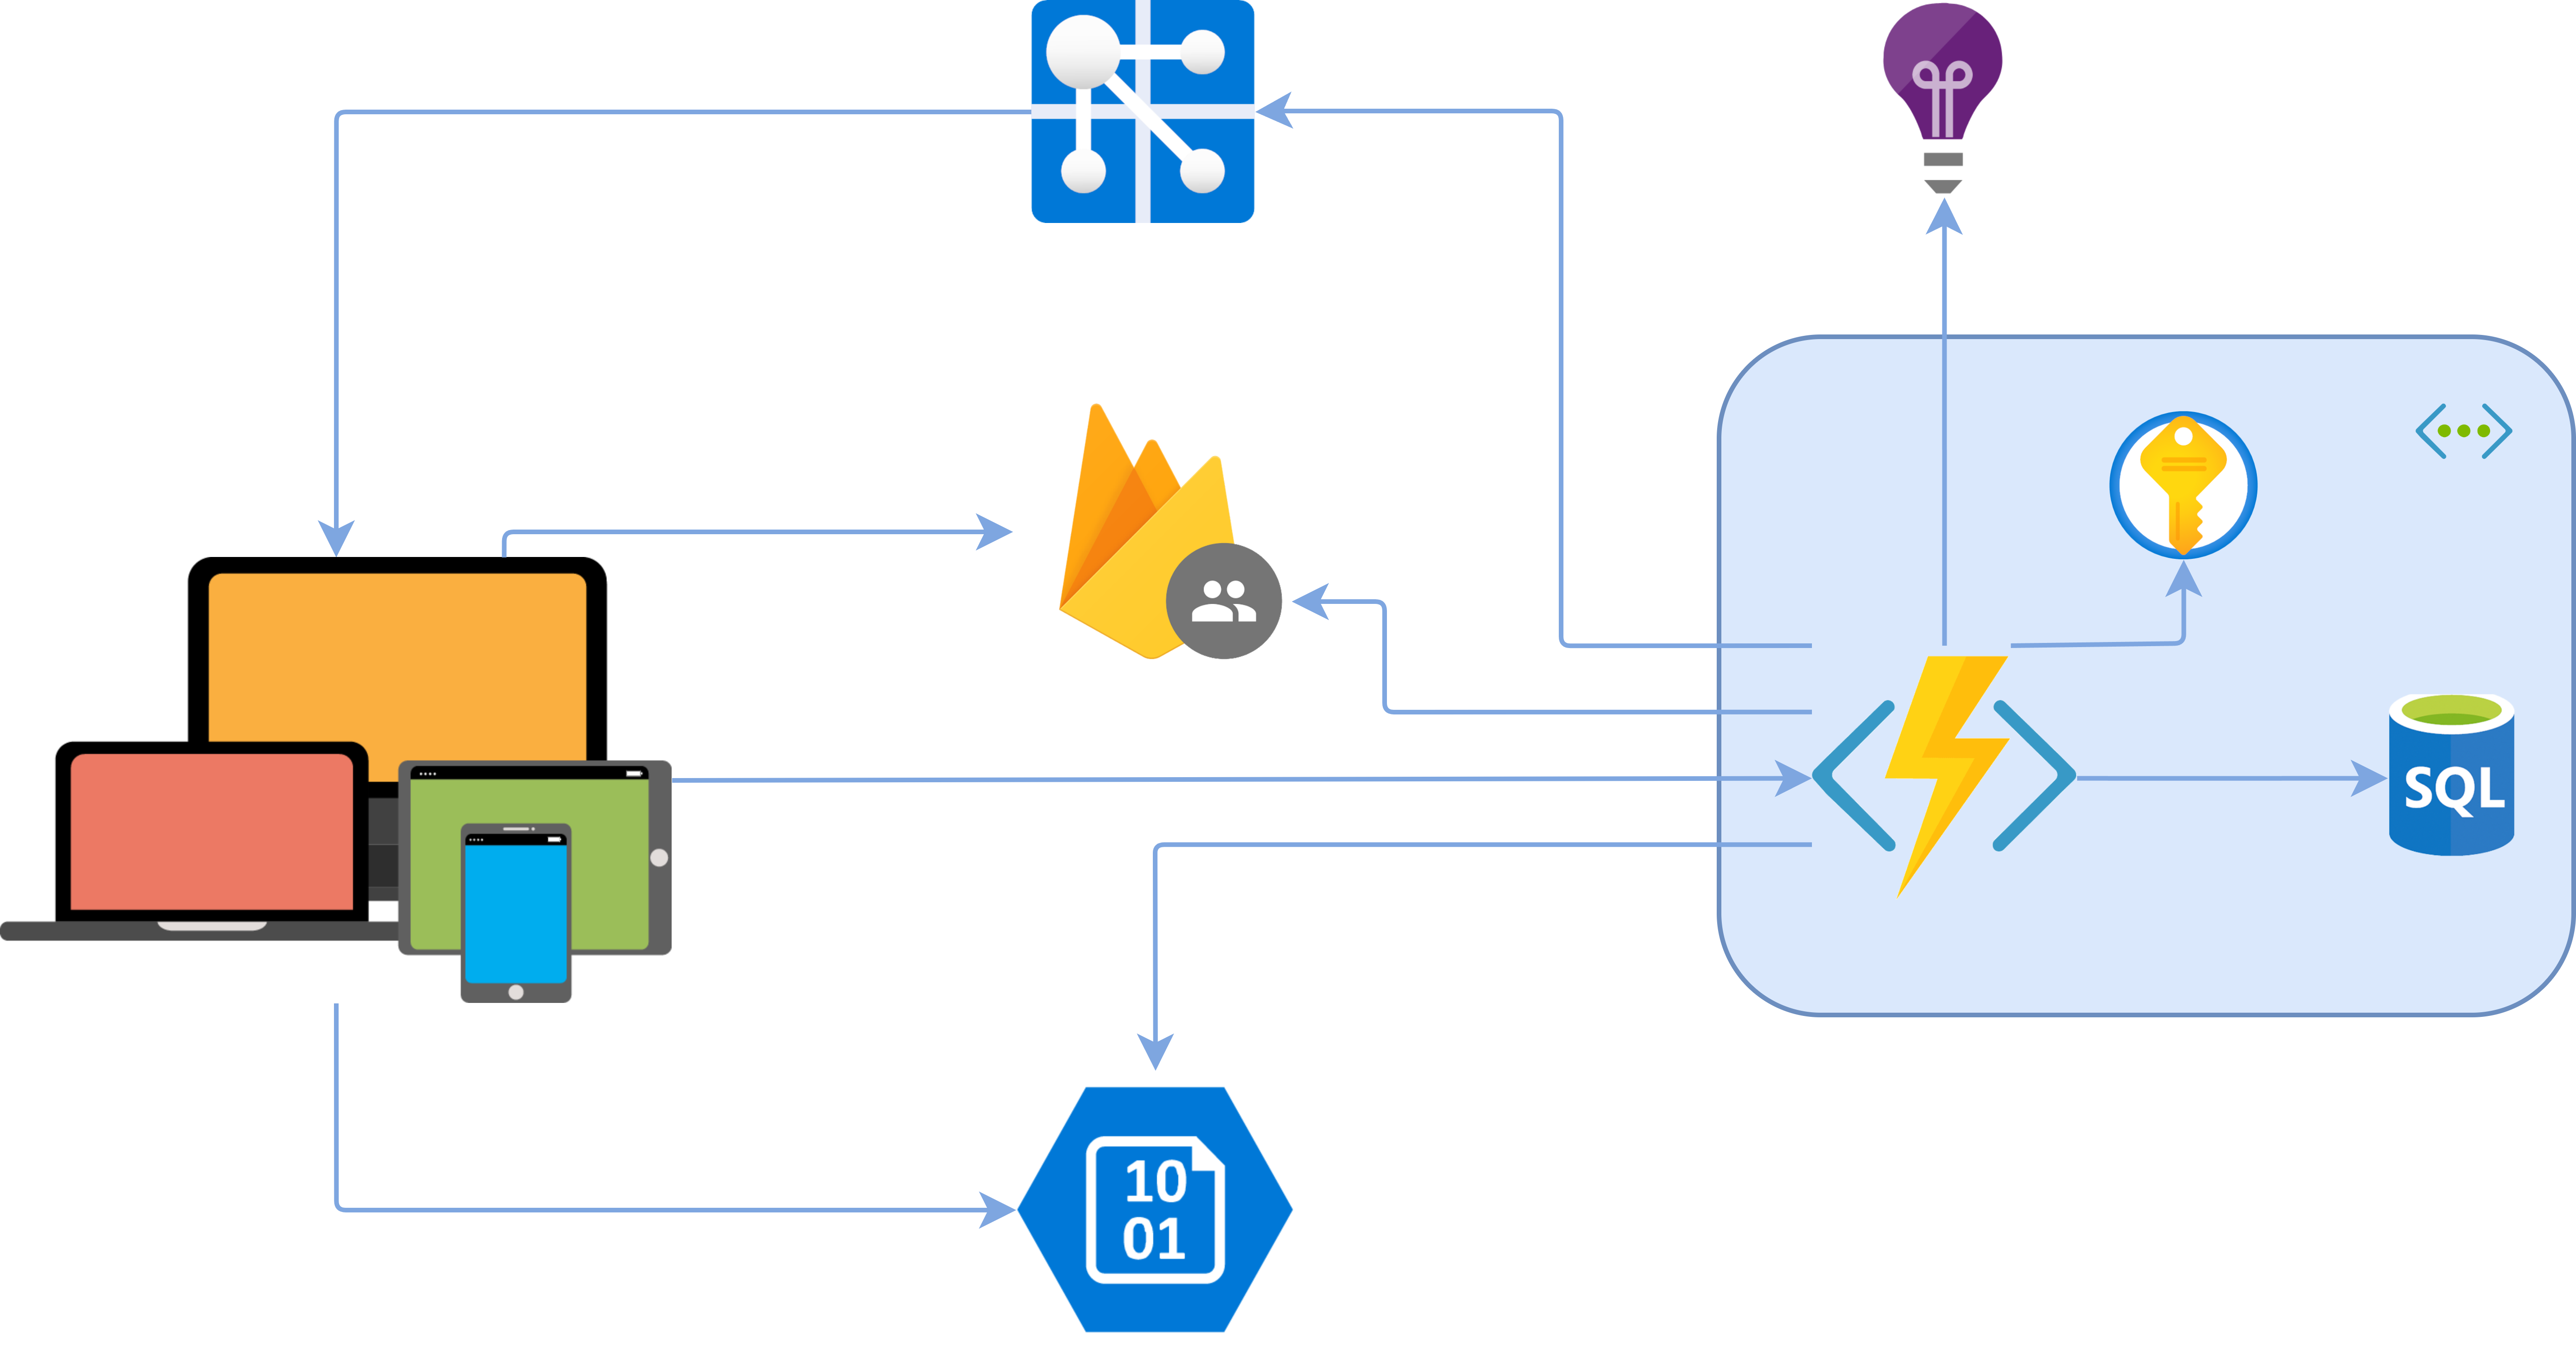
\includegraphics[width=\textwidth]{ImplementazioneArchitettura.png}
        \caption{Grafico dell'architettura di WYD}
    \end{center}
\end{figure}
\clearpage

\section{Sviluppi futuri}
Gli sviluppi futuri potranno comprendere, in base a decisioni di marketing:
\begin{itemize}
    \item La visualizzazione degli impegni degli altri profili
    \item L'implementazione di una chat per ogni gruppo
    \item Sviluppo di strumenti utili all'organizzazione dei gruppi, quali:
          \begin{itemize}
              \item form per combinare le disponibilità reciproche
              \item appunti condivisi(liste della spesa o note su chi porta cosa)
              \item calcolo delle spese compiute da ciascun componente
          \end{itemize}
    \item La creazione di profili pubblici che possono essere seguiti
    \item La creazione di eventi pubblici
    \item Una funzionalità di ricerca degli eventi o dei profili pubblici
    \item Supporto alla gestione di prenotazione e organizzazione degli eventi, dalle liste di attesa alla vendita dei biglietti
    \item La possibilità per le aziende di gestire in locale il proprio server e i relativi dati
\end{itemize}
\clearpage

\chapter*{Fonti bibliografiche e sitografia}
\addcontentsline{toc}{chapter}{Fonti bibliografiche e sitografia}

Object Management Group, OMG Unified Modelling Language Version 2.5.1, December 2017, https://www.omg.org/spec/UML/2.5.1/PDF

https://learn.microsoft.com/en-us/azure/reliability/reliability-cosmos-db-nosql
https://learn.microsoft.com/en-gb/azure/cosmos-db/throughput-serverless
https://learn.microsoft.com/en-gb/azure/cosmos-db/provision-throughput-autoscale